\documentclass[]{article}
\usepackage[T1]{fontenc}
\usepackage[utf8]{inputenc}
\usepackage{lmodern}
\usepackage[a4paper]{geometry}
\usepackage{babel}

\usepackage{amsmath}
\usepackage{amssymb}
\usepackage{graphicx}
\usepackage{url}
\usepackage{float}



\begin{document}
	
\thispagestyle{plain}
\begin{figure}[!h]
	\centering
	\begin{minipage}{0.45 \linewidth}
		\centering
		\LARGE{GAUTHIER Jeanne}\\
		\LARGE{MASSIN Keryann}
	\end{minipage}
	\hfill
	\begin{minipage}{0.48 \linewidth}
		\centering
		\Large{ENSAE 2nd year}\\
		\Large{Linear Time Series Project}		
	\end{minipage}
\end{figure}

\bigskip
\bigskip
\bigskip
\bigskip
\bigskip
\bigskip

\hrule
\begin{center}
	\Huge{Analysis of the French Industrial Production Index}
\end{center}
\hrule

\bigskip
\bigskip

\begin{figure}[h!]
	\centering
	
\includegraphics[scale=0.6]{ENSAE_logo.png}
\end{figure}
\bigskip
\bigskip
\bigskip
\begin{center}
	\today
\end{center}

\newpage
\tableofcontents

\newpage
\section{Part I: the data}
\subsection{Question 1}
\textit{What does the chosen series represent ? (sector, potential data processing, logarithmic transformation, etc.)}\\

In this project, we will take a look at the French Industrial Production Index (IPI), available on INSEE website at this link: \url{https://www.insee.fr/fr/statistiques/serie/010537206}.
This series is corrected from seasonal variations and working days, on a monthly frequency and makes it possible to follow the monthly evolution of industrial activity in France and in construction.\\
The initial series records the IPI from January 1990 to to March 2023 (base 100 in 2015). It is plotted on figure \ref{rawSeries} below:
\begin{figure}[h!]
	\centering
	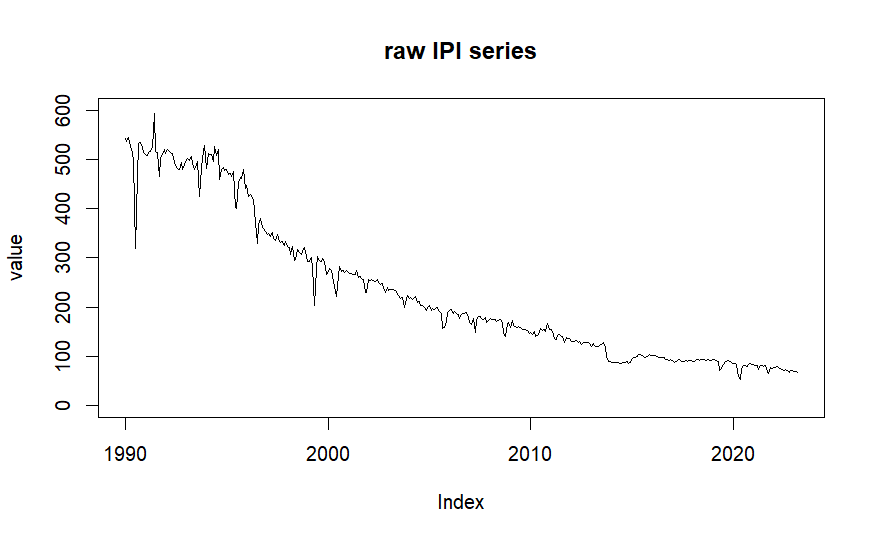
\includegraphics[scale=0.6]{raw_series.png}
	\caption{Raw initial series of French Industrial Production Index}
	\label{rawSeries}
\end{figure}\\
As the series is already corrected from seasonal variations and working days, these data processing are unnecessary. However, the series' empirical variance seems proportional to its values. We correct this effect (thus diminishing heteroskedasticity) by applying a Box Cox transformation of parameter $\lambda = 0$. Namely, we take the logarithm, to obtain figure \ref{logSeries}.
\begin{figure}[h!]
	\centering
	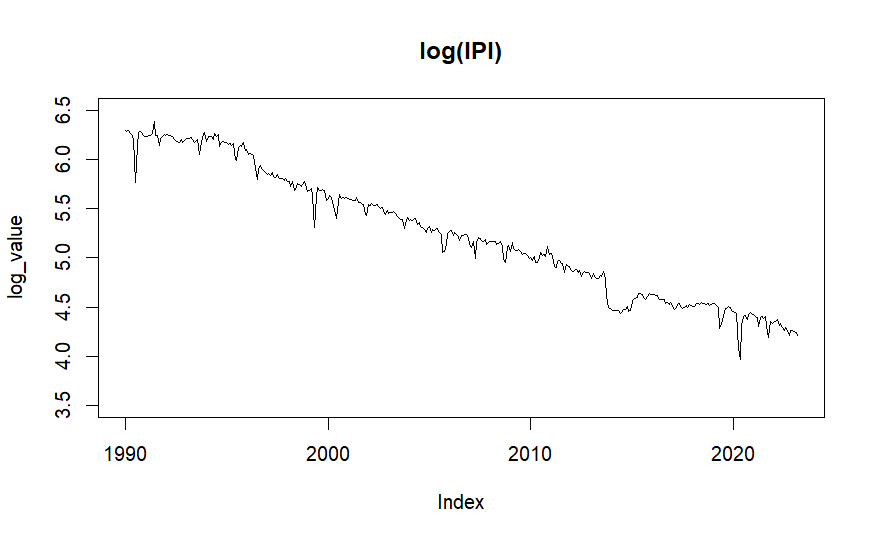
\includegraphics[scale=0.6]{log_series.png}
	\caption{logarithm of IPI}
	\label{logSeries}
\end{figure}


\subsection{Question 2}
\textit{Transform the series to make it stationary if necessary (differentiate it, correct the deterministic trend, etc.). Thoroughly justify your choices.}\\

Clearly, figure \ref{logSeries} shows that log(IPI) is not stationary. To statistically back this affirmation, we conducted Augmented Dickey-Fuller and KPSS tests both on log(IPI) and on the first difference of log(IPI). Table \ref{ADFandKPSS} shows the results.\\

The Augmented Dickey-Fuller test rejects the null hypothesis of non-stationarity for the first difference of log(IPI) at the $1\%$ level and does not reject it for log(IPI) at the $5\%$ level.\\

The KPSS test rejects the null hypothesis of stationarity for log(IPI) at the $1\%$ level but does not reject it for the first difference of log(IPI) at the $10\%$ level.\\

As a result of these two tests, we can confidently argue that our corrected time series 'First difference of log(IPI)' (see figure \ref{stationarySeries}) is stationary. Therefore, log(IPI) was indeed a I(1).

\begin{table}[!h]
	\centering
	\begin{tabular}{|c||c|c|}
		\hline
		& ADF p-value & KPSS p-value\\
		\hline
		\hline
		log(IPI) & 0.06 & 0.01\\
		\hline
		first difference of log(IPI) & 0.01 & 0.1\\
		\hline
	\end{tabular}
	\caption{ADF and KPSS tests for stationarity}
	\label{ADFandKPSS}
\end{table}

\subsection{Question 3}
\textit{Graphically represent the chosen series before and after transforming it.}\\

We can finally compare our two series: the initial raw series and the stationarized one. We plotted them in figures \ref{rawSeries2} and \ref{stationarySeries}.
\begin{figure}[!h]
	\centering
	\begin{minipage}{0.45 \linewidth}
		\centering
		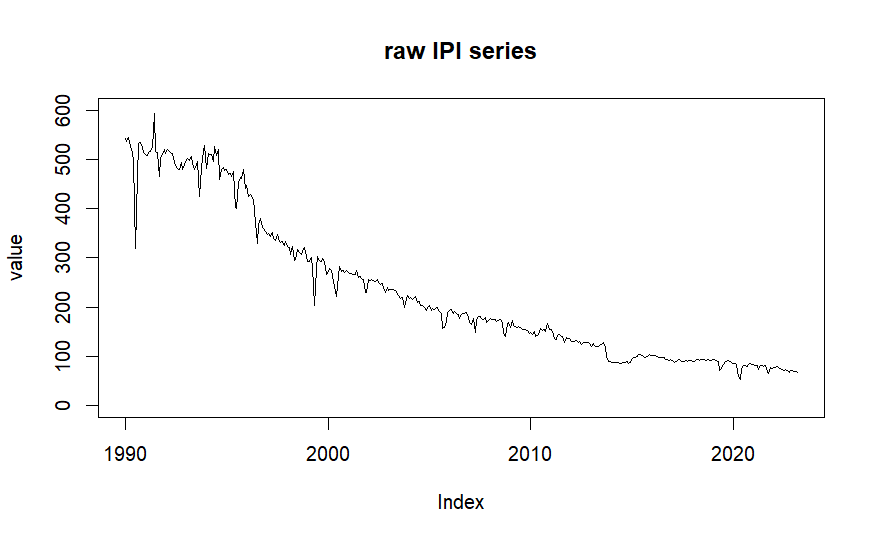
\includegraphics[scale=0.4]{raw_series.png}
		\caption{Raw initial series of French Industrial Production Index}
		\label{rawSeries2}
	\end{minipage}
	\hfill
	\begin{minipage}{0.48 \linewidth}
		\centering
		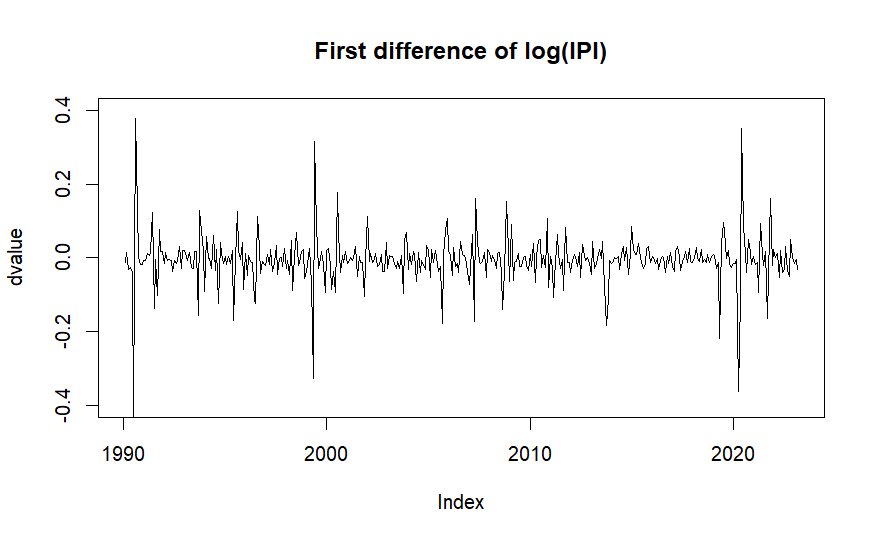
\includegraphics[scale=0.4]{stationary_series.png}
		\caption{Corrected time series}
		\label{stationarySeries}
	\end{minipage}
\end{figure}\\

\newpage
\section{Part II:  ARMA models}

\subsection{Question 4}
\textit{Pick (and justify your choice) an ARMA(p, q) model for your corrected time series $X_t$. Estimate the model parameters and check its validity.}\\

In this part, we will attempt to find the ARMA(p, q) model that best fits our corrected time series $X_t$ (see figure \ref{stationarySeries}). We assume stationarity of $X_t$. To select the right model, we will first take a look at autocorrelation function (ACF) and partial autocorrelation function (PACF). This will allow us to find maximal orders $p_{max}$ and $q_{max}$ of the ARMA(p, q) model. To evaluate $p_{max}$ (resp. $q_{max}$), we analyze PACF (resp. ACF).
\begin{figure}[!h]
	\centering
	\begin{minipage}{0.45 \linewidth}
		\centering
		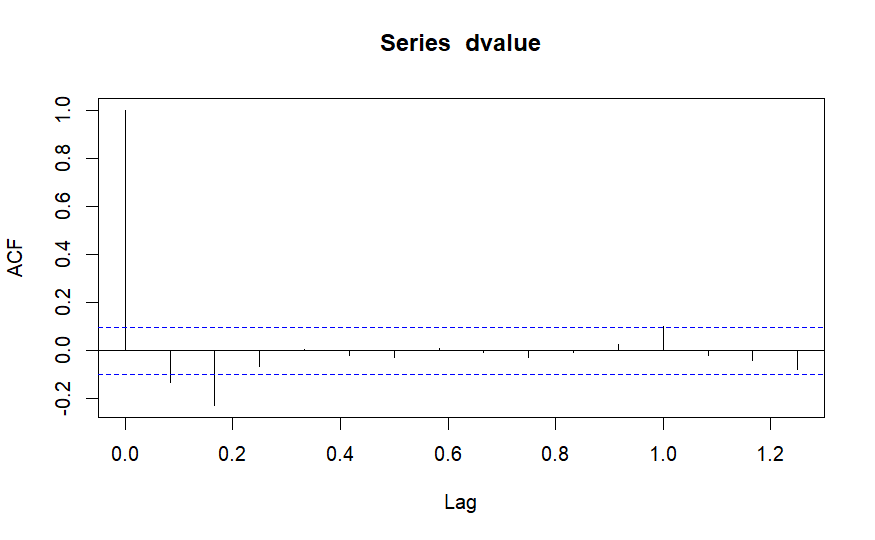
\includegraphics[scale=0.4]{ACF.png}
		\caption{Autocorrelation function}
		\label{ACFplot}
	\end{minipage}
	\hfill
	\begin{minipage}{0.48 \linewidth}
		\centering
		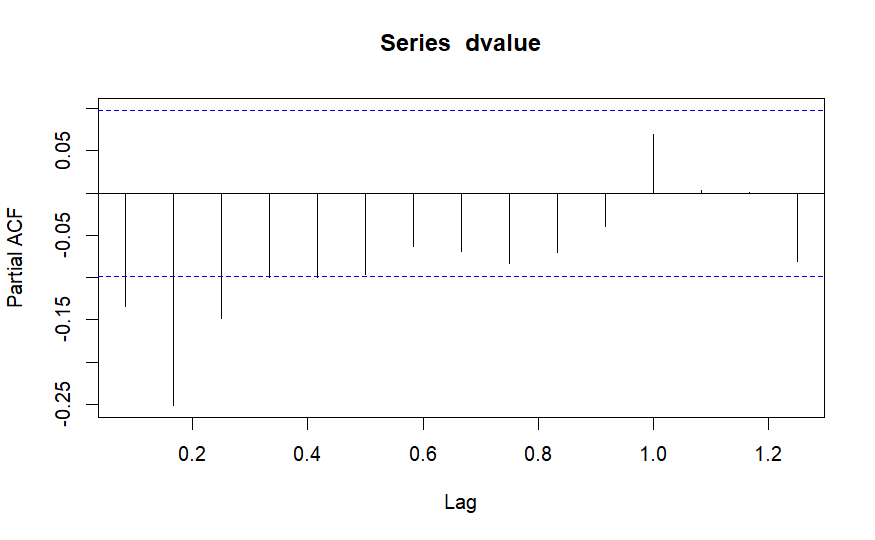
\includegraphics[scale=0.4]{PACF.png}
		\caption{Partial autocorrelation function}
		\label{PACFplot}
	\end{minipage}
\end{figure}
On figures \ref{ACFplot} and \ref{PACFplot}, we see that empirical autocorrelations and partial autocorrelations decrease rapidly. Hence, an ARMA(p, q) can rightfully be fitted on the series.\\
From figure \ref{ACFplot}, we see that autocorrelation is statistically different from $0$ for lags $0, 1, 2$, so we pick $q_{max}=2$. From figure \ref{PACFplot}, we see that partial autocorrelation is statistically different from $0$ for lags $1, 2, 3$ so we pick $p_{max}=3$.\\

We are therefore looking for an ARMA(p, q) model that satisfies three conditions:
\begin{itemize}
	\item $p\in \{0, 1, 2, 3 =p_{max}\}$ and $q\in \{0, 1, 2=q_{max}\}$
	\item The model is valid, which means that its residuals are not autocorrelated.\\
	We can check it using the Ljung-Box test with null hypothesis being the joint nullity of autocorrelations until order $k$. We chosed $k=24$.
	\item The model is well-adjusted, which means that its coefficients are statistically significant.\\
	We can check it using the usual approach to test the significance of a linear regression's coefficients, the t-Student test.
\end{itemize}
From the twelve possible models, only three are valid and well-adjusted: ARMA(2, 1), MA(2) and ARMA(1, 2). To chose the best fitted, we compare their AIC and BIC in table \ref{AICvsBIC}.
\begin{table}[!h]
	\centering
	\begin{tabular}{|c||c|c|c|}
		\hline
		      & \text{ARMA(2, 1)} & \text{MA(2)} & \text{ARMA(1, 2)}\\
		\hline
		\hline
		AIC & -1078.649 & -1075.884 & -1079.288\\
		\hline
		BIC & -1058.717 & -1059.938 & -1059.356\\
		\hline
	\end{tabular}
	\caption{AIC and BIC for the different ARMA(p, q) models}
	\label{AICvsBIC}
\end{table}\\
According to table \ref{AICvsBIC}, AIC and BIC are respectively minimized for ARMA(1, 2) and MA(2) models. In addition, the ARMA(1, 2) model presents a BIC close to the MA(2) model's. We thus consider that ARMA(1, 2) is the best fit for $X_t$.

\subsection{Question 5}
\textit{Write the ARIMA(p,d,q) model for the chosen series.}\\

For $(p, d, q) = (1, 1, 2)$, the model is well-adjusted (the coefficients are significant) and is valid (the residuals are not autocorrelated), so our series log(IPI) (see figure \ref{logSeries}) fits with an ARIMA(1,1,2).\\
Let $Y_t$ be our raw series in figure \ref{rawSeries}. With $X_t  = \log(Y_{t}) - \log(Y_{t-1})$, $\epsilon_t$ the residuals at time $t$, and by evaluating the coefficients of the model, we finally have:
\begin{equation}
	X_t = 0.208 X_{t-1} + \epsilon_t - 0.426 \epsilon_{t-1} - 0.214 \epsilon_{t-2}
\end{equation}


\section{Part III: Prediction}
\textit{Denote T the length of the series. Assume the series residuals are Gaussian.}\\

In the following, we denote $T$ the length of the series and we assume the series residuals are gaussian, that is $\epsilon_t \sim \mathcal{N}(0, \sigma^2)$ with $\sigma^2>0$. We have a ARMA(1,2) which translates:
\begin{equation}
	\label{arma12equation}
	X_t = \phi_1 X_{t-1} + \epsilon_t + \theta_1 \epsilon_{t-1}+ \theta_2 \epsilon_{t-2}
\end{equation}



\subsection{Question 6}
\textit{Write the equation satisfied by the confidence region of level $\alpha$ on the future values $(X_{T+1}, X_{T+2})$.}\\

Given $\mathbb{E}[\epsilon_{T+h}\mid X_T, X_{T-1},\dots] = 0,\; \forall h>0$, optimal predictions satisfy:
\begin{equation}
	\left\{
	\begin{array}{ll}
		&\hat{X}_{T+1\mid T} = \phi_1 X_{T} + \theta_1 \epsilon_{T}+ \theta_2 \epsilon_{T-1}\\
		&\hat{X}_{T+2\mid T} = \phi_1 \hat{X}_{T+1\mid T} + \theta_2 \epsilon_{T}
	\end{array}\right.
\end{equation}
Let us calculate prediction erros $X_{T+1} - \hat{X}_{T+1\mid T}$ and $X_{T+2} - \hat{X}_{T+2\mid T}$. It writes:
\begin{equation}
	\hat{X} = 
	\begin{pmatrix}
		\hat{X}_{T+1\mid T}\\
		\hat{X}_{T+2\mid T}
	\end{pmatrix}\quad
	\text{and}\quad
	X = \begin{pmatrix}
		X_{T+1}\\
		X_{T+2}
	\end{pmatrix}
\end{equation}
Thus, using \eqref{arma12equation}:
\begin{equation}
	X - \hat{X} = 
	\begin{pmatrix}
		X_{T+1} - \hat{X}_{T+1\mid T}\\
		X_{T+2} - \hat{X}_{T+2\mid T}
	\end{pmatrix}
	=
	\begin{pmatrix}
	\epsilon_{T+1}\\
	\epsilon_{T+2} + (\phi_1 + \theta_1)\epsilon_{T+1}\\
	\end{pmatrix}
\end{equation}
We can now compute the variance of prediction errors:
\begin{equation}
	\left\{
	\begin{array}{ll}
		&\mathbb{V}(X_{T+1} - \hat{X}_{T+1\mid T}) = \mathbb{V}(\epsilon_{T+1}) = \sigma^2\\
		&\mathbb{V}(X_{T+2} - \hat{X}_{T+2\mid T}) = \mathbb{V}(\epsilon_{T+2} + (\phi_1 + \theta_1)\epsilon_{T+1}) = \sigma^2(1+(\phi_1 + \theta_1)^2)
	\end{array}
	\right.
\end{equation}
$X-\hat{X}$ thus follows a normal distribution of mean $\mu = 0$ and variance $\Sigma$, that is:
\begin{equation}
	X-\hat{X} \sim \mathcal{N}(0, \sigma^2) \quad \text{where}\quad
	\Sigma = \sigma^2
	\begin{pmatrix}
	1 & \phi_1 + \theta_1\\
	\phi_1 + \theta_1 & 1 + (\phi_1 + \theta_1)^2
	\end{pmatrix}
\end{equation}
We see that $\det(\Sigma) = \sigma^2$, so $\Sigma$ is invertible if and only if $\sigma^2>0$, which is true by assumption.
According to the lectures, we finally have $(X-\hat{X})^T\Sigma^{-1}(X-\hat{X}) \sim \chi^2(2)$. It follows that the confidence region $R_{\alpha}$ of level $\alpha$ verifies, for all $\alpha\in [0,1]$:
\begin{equation}
	R_{\alpha} = \{X\in \mathbb{R}^2\mid (X-\hat{X})^T\Sigma^{-1}(X-\hat{X}) \leq q_{\chi^2(2)}^{1-\alpha}\}
\end{equation}
where $q_{\chi^2(2)}^{1-\alpha}$ is the $(1-\alpha)$-quantile of $\chi^2(2)$ distribution.
\subsection{Question 7}
\textit{Give the hypothesis used to get this region.}\\

To get the previous results, we made some hypothesis:
\begin{itemize}
	\item The model is perfectly known
	\item The coefficients obtained in part $2$ are correct
	\item The white noise follows a normal distribution $\epsilon_t \sim \mathcal{N}(0, \sigma^2)$
	\item $\sigma^2 > 0$
\end{itemize}

\subsection{Question 8}
\textit{Graphically represent this region for $\alpha = 95\%$. Comment on it.}\\



\subsection{Question 9 -  Open question}
\textit{Let $Y_t$ a stationary time series available from $t=1$ to $T$. We assume that $Y_{T+1}$ is available faster than $X_{T+1}$. Under which condition(s) does this information allow you to improve the prediction of $X_{T+1}$? How would you test it/them?}\\

Under the assumption that $Y_{T+1}$ is available faster than $X_{T+1}$, we can use $Y_{T+1}$ to predict $X_{T+1}$ if and only if
\begin{equation}
	\hat{X}_{T+1\mid \{X_t, Y_t\mid t<T\}\cup \{Y_{T+1}\}} \ne \hat{X}_{T+1\mid \{X_t, Y_t\mid t<T\}}
\end{equation}
i.e if and only if $Y_t$ instantaneously causes $X_t$ in the Granger sense.

\end{document}
